\section{Роль и обязанности специалиста по защите информации.}
\subsection{Защита от внешних угроз.}
    Одной из обязанностей специалиста в данной сфере является защита передаваемой информации от потенциальной фальсификации. Вопросами, связанными с конфиденциальностью и 
    сохранностью передаваемой информации, занимается
    \textbf{криптография.} Это раздел математики, ассоциирующийся с кодированием данных, однако это не совсем так.
    Помимо этого, криптография также охватывает вопросы, связанные с подменностью цифровых данных, а именно: проверка достоверности
    цифровых данных, верификация этих данных.

    Примером такого механизма защиты данных является \textbf{электронная цифровая подпись(ЭЦП)}. ЭЦП "--- реквизит электронного документа, предназначенный для 
    защиты данного документа от подделки, полученный в результате криптографического преобразования
    информации с помощью закрытого ключа электронной цифровой подписи. ЭЦП позволяет идентифицировать владельца сертификата
    ключа подписи. Помимо этого, ЭЦП является необходимым атрибутом любого электронного документа и делается в виде специально
    закодированной строки при помощи новейших технологий.  

    Электронная цифровая подпись состоит из 3"=х основных элементов:

    \begin{enumerate}
        \item Сертификат;
        \item Открытый ключ;
        \item Закрытый ключ.
    \end{enumerate}

    В сертификате находится краткая информация о владельце, а ключи состоят из закодированных символов. Более подробное описание механизма работы ЭЦП можно увидеть на рисунке 4.1. 

    \begin{figure}[H]
        \centering
        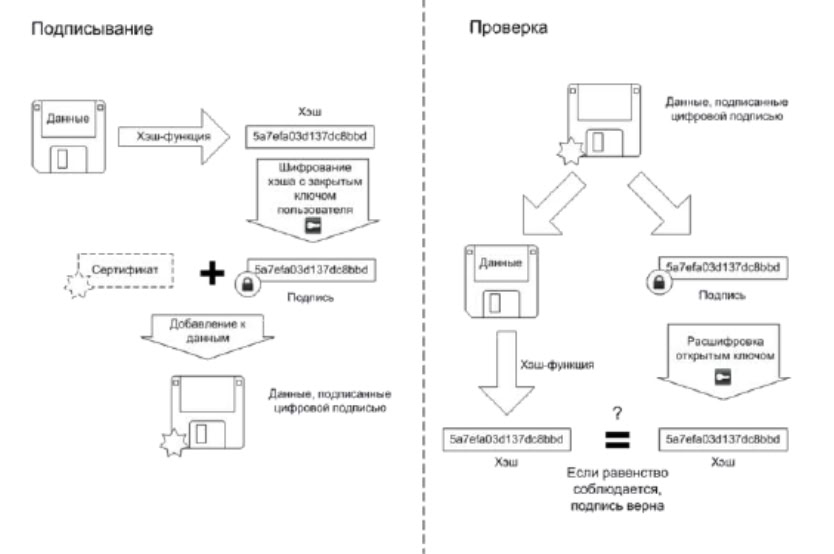
\includegraphics[height = 11cm, width = 14cm]{pic/legit_doc.png}
        \caption{Пример работы ЭЦП}
    \end{figure}

    ЭЦП была произведена для исполнения сделок различного рода между юридическими лицами в интерактивном режиме,
    а также для обмена важной информацией, которая нуждается в конфиденциальности. За счёт криптографического преобразования,
    документ имеет ряд символов, которые возникают посредством работы ПО, создающего электронную подпись. Таким образом, данный документ
    может открыть только тот пользователь, которому он был отправлен.

    Исходя из вышесказанного, ЭЦП даёт гарантию, что авторское право документа не подлежит фальсификации\cite{crypto}.

\newpage
\subsection{Мониторинг систем информационной безопасности.}
    Безопасность информационных систем основывается на защите систем от уязвимостей, которые в свою очередь могут возникать из"=за
    ошибок в конфигурации компонентов информационной системы. \textbf{Мониторинг информационной безопасности} представляет собой процесс систематического 
    наблюдения, анализа и контроля за состоянием безопасности информационных систем и данных. Дерево архитектуры системы мониторинга изображено на рисунке 4.2. Он осуществляется с помощью специализированных программных и 
    аппаратных средств, которые позволяют выявлять, предотвращать и реагировать на возможные угрозы, нарушения и аномалии в информационной среде организации.
    Основная цель мониторинга "--- обнаружение ошибок конфигурации и инцидентов в режиме реального времени, чтобы минимизировать ущерб для конкретной компании.
    Помимо этого, мониторинг информационной безопасности позволяет предотвратить возможные атаки.

    \begin{figure}[H]
        \centering
        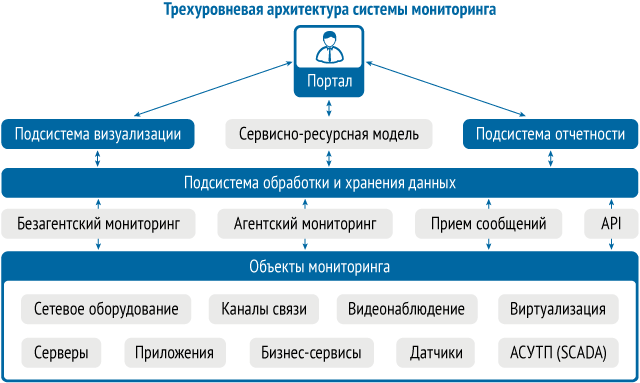
\includegraphics[width = 14cm]{pic/monitoring.png}
        \caption{Дерево мониторинга систем}        
    \end{figure}

    \newpage
    Мониторинг систем информационной безопасности является комплексным процессом, который выполняется в несколько этапов:

    \begin{enumerate}
        \item \textbf{Сбор данных и логов.}
            Мониторинг начинается со сбора данных из различных информационных систем. Эти данные представляют основу для анализа безопасности;
        \item \textbf{Анализ данных.}
            Собранные данные проходят через определенные алгоритмы анализа данных с целью выявления различных угроз или аномалий;
        \item \textbf{Обнаружение инцидентов.}
            На данном этапе мониторинг позволяет выявить различные угрозы, что позволяет оперативно среагировать на них;
        \item \textbf{Реагирование на инциденты.}
            Команда специалистов по обеспечению безопасности должна иметь определенный план реагирования для различных сценариев. Мониторинг
            в свою очередь помогает минимизировать ущерб от атак;
        \item \textbf{Отчет и анализ производительности.}
            Мониторинг систем информационной безопасности также включает в себя анализ эффективности применяемых мер и создание отчётов о безопасности\cite{monitoring}.
    \end{enumerate}

    Однако несмотря на уровень профессионализма специалистов, всё равно периодически происходят атаки на информационные системы. В этом случае, специалист 
    должен провести процедуру \textbf{восстановления после атаки.} 

\newpage
\subsection{Восстановление после атак. Резервное копирование информации.}
    \textbf{Кибератака} (или атака на информационную систему) "--- комплекс действий, нацеленный на нарушение доступности и конфиденциальности информации.
    Успешная кибератака может привести к существенной утечке данных и важной информации компании.
    В случае, если атака всё же произошла, специалисту по защите информационной безопасности необходимо разработать сценарий действий и согласовать его 
    с остальными сотрудниками. В зависимости от <<силы>> проведённой атаки может потребоваться значительное количество средств и времени на восстановление.

    Рассмотрим один из самых популярных методов восстановления информации "--- восстановление через \textbf{резервное копирование}. Само резервное копирование 
    может проводиться с помощью физического носителя (например, жесткий диск), облачного хранилища, или с помощью гибридного метода, подразумевающего использование
    как и физического носителя, так и облачного хранилища. В зависимости от ресурсов кампании и согласованного сценария, применяется один из этих методов восстановления.
    Резервное копирование может осуществляться различными способами. В этой статье будут рассмотренны основные и самые популярные\cite{main_methods}.

    \textbf{Полное резервное копирование} "--- копирование абсолютно всей информации. С его помощью можно восстановить всю информацию в любой момент времени. Основным минусом
    этого метода является требуемый объём памяти. Помимо этого, восстановление данных этим методом предполагает полную замену, что может занять значительное время.

    \textbf{Инкрементальное резервное копирование} "--- процесс копирования, при котором старые (т.е. уже сохраненные) данные остаются без изменений, а новые данные,в том числе и утерянные, 
    восстанавливаются. При использовании данного метода, создаются несколько копий данных, а именно нулевая и инкрементные копии, где нулевая копия является полной.

    \textbf{Дифференциальное резервное копирование} "--- данный процесс использует разницу между двумя версиями данных. Первоначально создаётся полная копия, затем копируются изменения.

    В зависимости от выбранного метода восстановления, определяются ресурсы и время, необходимые для полного восстановления.


\newpage
\subsection{Обучение сотрудников правилам безопасности.}

    В период восстановления после атак активно продумывается каждый этап восстановления, в том числе и снижение будущих
    потенциальных рисков подобных угроз. Одним из самых важных аспектов восстановления является обучение сотрудников правилам безопасности.
    
    В зависимости от масштаба, причины и метода произведённой атаки, специалист обязан провести обучение с целью подготовить сотрудников фирмы 
    к подобным атакам. Его задача - предотвратить использование определённого ПО сотрудниками в случае, если причиной атаки стало именно оно,
    подготовить и согласовать сценарий действий в случае, если подобная атака повторится ещё раз. Помимо этого, специалист должен выработать
    определённые правила конфиденциальности информации в фирме на время уязвимости после произведённой атаки.




